 
   %judul bisa diketik ulang
  \setstretch{1}%\small
  \begin{center}
      \textbf{\large \Title}\\
      \bigskip 
  \end{center}
  
  
  
  %Nama authors
   \begin{center}
     \bf \Author$^1$, Mira Kania Sabariah$^2$, Monterico Adrian$^3$
  \end{center}
  
  
  %Afiliasi dan email
   \begin{center}
     $^{1,2,3}$Fakultas Informatika, Universitas Telkom, Bandung\\
$^4$Divisi Digital Service PT Telekomunikasi Indonesia\\
$^1$rovino@students.telkomuniversity.ac.id, $^2$mirakarnia@telkomuniversity.ac.id,\\ $^3$monterico@telkomuniversity.ac.id
  \end{center}
  
   
 %%% Abstrak Indonesia %%%%%%%%%%  
   
{\bf \parindent0pt \noindent\rule{\textwidth}{1pt}
Abstrak

Populasi penduduk yang tinggi di Indonesia mengakibatkan antrian panjang dalam berbagai pelayanan publik atau pelayanan konsumen. Pelanggan harus datang ke tempat untuk mengambil antrian dan menunggu gilirannya, semakin panjang antrian, semakin lama waktu tunggu yang dibutuhkan. Hal ini tidak efisien dan menyebabkan banyak waktu terbuang hanya untuk menunggu antrian. Jika nomor antrian bisa didapatkan secara online dan dapat dipantau secara online, maka dapat mengurangi waktu yang terbuang. Dengan aplikasi antrian virtual dapat memperpendek antrian secara fisik, dengan cara antri secara virtual, melihat antrian yang sedang berjalan, dan booking tempat. Pada Pengembangan aplikasi ini, framework yang digunakan adalah NestJS dan PrismaJS dengan menerapkan RESTful API, Object Relational Mapping, dan menghindari Anti-Pattern. Framework NestJS mendukung pembuatan aplikasi ber-arsitektur monolitik dan \textit{microservice}. Setelah aplikasi dibangun di arsitektur monolitik, aplikasi dapat dengan mudah dimigrasikan ke \textit{microservice} saat penggunaan aplikasi sudah hampir mendekati batas muat pengguna.\\

 \bigskip
Kata kunci : NestJS, PrismaJS, Anti-Pattern, Antrian, Backend, REST



%%% Abstrak English %%%%%%%%%%  



\noindent\rule{\textwidth}{1pt}
Abstract

The abstract should state briefly the general aspects of the subject and the main concolusions.  The length of abstract should bo no more than 200 word and  should be typed be with 10 pts.

 \bigskip
Keywords: keyword should be chosen that they best describe the contents of the paper and should be typed in lower-case, except abbreviation. Keyword should be no more than 6 word 

\noindent\rule{\textwidth}{1pt} }
   


%%%%%% isi paper %%%%

\section{Pendahuluan}

\noindent\textbf{Latar Belakang}

Meningkatnya populasi di indonesia mengakibatkan banyak pelanggan ya-ng mengantri untuk mendapatkan layanan di bank, restoran, rumah sakit, dan tempat penyedia jasa lainnya. Mengantri merupakan kegiatan yang membosankan dan menguras waktu. Panjangnya antrian juga mampu berdampak pada mutu pelayanan di suatu tempat. Pelanggan yang harus menunggu lama berpotensi beralih ke pesaing, atau jika ada urusan lain yang lebih penting, maka pelanggan akan keluar dari tempat antrian, meninggalkan antriannya \cite{khong2017queue}\cite{Ghazal2016}\cite{Uddin2016}. Solusi yang ada pada bank, kantor pos, dan rumah sakit saat ini menggunakan \textit{ticketting} nomor antrian secara manual, dimana antrian yang sedang dilayani ditampilkan di layar pada ruang tunggu. Hal ini kurang efektif karena pelanggan harus berada di ruang tunggu\cite{Ghazal2016}.

Perkembangan teknologi yang cepat mengakibatkan penggunaan perangkat pintar atau \textit{smartphone} merupakan hal lumrah, banyak bermunculan aplikasi antrian virtual seperti Antrique, Qiwee, ExaQue dimana pengguna dapat mengantri dari jarak jauh melalui aplikasi maupun \textit{website}. Para pengguna aplikasi tersebut dapat melakukan hal lain saat mengantri sebelum gilirannya. Namun, aplikasi-aplikasi tersebut memiliki banyak kelemahan seperti \textit{UI/UX} yang tidak bagus, sering \textit{crash} dan \textit{freeze}, tidak ada estimasi waktu antrian, dan masih belum ada yang berfokus ke sektor \textit{food and beverage}.

Oleh karena itu, perlunya dikembangkan sebuah aplikasi yang memiliki fitur yang sama atau lebih dengan menutup kekurangan pada aplikasi tersebut. Pengembangan aplikasi yang direncanakan menggunakan arsitektur monolitik karena mudahnya untuk dibuat dan di-\textit{deploy} secara cepat untuk di iterasikan. Namun, arsitektur monolitik memiliki kelemahan seperti sulitnya untuk di-\textit{maintenance}, \textit{scale}, dan reliabilitas nya. Oleh karena itu, perlu diperhatikan bagaimana cakupan aplikasi kedepannya dan perlunya migrasi ke arsitektur \textit{microservice} \cite{gos2020comparison} \cite{jatkiewicz2023differences}.

Dalam pengembangan aplikasi web, pemilihan bahasa pemrograman untuk digunakan di \textit{backend} sangatlah penting karena dapat mempengaruhi performa aplikasi yang dibangun. Dalam pemilihan bahasa pemrograman \textit{backend}, banyak pilihan yang tersedia seperti PHP, Python, Ruby, PERL, dan banyak lagi. NodeJs merupakan \textit{tools} yang memungkinkan bahasa JavaScript dapat dijalankan pada sisi \textit{backend}. Dalam sisi performa, NodeJs lebih unggul dibanding PHP dan Python dalam sisi kecepatan melayani \textit{request} dari client \cite{William2020} \cite{Odeniran2023}.

NestJs merupakan \textit{framework backend} dari Nodejs yang menggunakan bahasa typescript, dan bisa digunakan untuk pengembangan arsitektur berbasis \textit{microservice} dan monolitik, jadi jika aplikasi dikembangkan pada arsitektur monolitik dapat dengan mudah dimigrasikan ke \textit{microservice}. NestJs juga bisa digunakan bersamaan dengan \textit{framework} PrismaJs untuk mengelola database \cite{NestJS}. PrismaJs merupakan \textit{framework} Object Relational Mapping (ORM) \cite{Prisma}, digunakan untuk mempercepat, dan mempermudah pengembangan aplikasi yang database-nya memiliki relasi yang kompleks dan sulit di-\textit{maintenance} jika menggunakan Structured Query Language (SQL) \cite{Zmaranda2020}.

Implementasi Application Programming Interface (API) yang digunakan adalah Representational State Transfer (RESTful) API, RESTful API adalah arsitektur untuk mempermudah komunikasi client-server agar efektif untuk transaksi data. Namun, pada implementasi RESTful API, ada beberapa hal yang perlu diperhatikan seperti keamanan saat transaksi  atau komunikasi \cite{Beer2018}. Keamanan yang lemah dapat mengakibatkan hacker dapat dengan mudah melakukan \textit{request tampering}, mengambil data pengguna, dan dapat membocorkan data keuangan mitra. \textit{Design pattern} juga perlu diperhatikan dalam penggunaan bahasa untuk API \textit{endpoint} nya agar tidak terjadi \textit{anti pattern}. \textit{Anti pattern} terjadi saat penamaan API tidak sesuai dengan fungsi, atau ada fungsi sejenis tapi penamaannya berbeda jauh. Dengan menghindari \textit{anti pattern}, dapat berakibat ke aplikasi yang lebih mudah di-\textit{sustain} dan di-\textit{maintain} \cite{Aghajani2018} \cite{Alshraiedeh2021}.

Berdasarkan uraian di atas, penelitian ini akan membuat sebuah \textit{backend} aplikasi antrian dengan menggunakan arsitektur monolitik dengan \textit{framework} NestJs dan PrismaJs sebagai \textit{framework} nya. Setelah fitur-fitur aplikasi dibuat, perlu dilakukan unit testing untuk memvalidasi kodingan yang telah ditulis. Hal ini bertujuan untuk meminimalisir bug dan mencegah terjadinya regresi saat fitur baru ditambahkan \cite{runeson2006survey}.\\

\noindent\textbf{Topik dan Batasannya}

Aplikasi antria memerlukan backend developer untuk mengimplementasi-kan fungsi fungsi API dan manajemen database nya. Maka dapat dirumuskan permasalahan sebagai berikut:
\begin{enumerate}
  \item Bagaimana meningkatkan \textit{sustainability} dan \textit{maintainability} pada penggunaan manajemen database.
  \item Bagaimana merancang API yang bebas dari \textit{anti pattern}.
  \item Bagaimana merancang sistem keamanan pada API untuk melayani \textit{request}.
\end{enumerate}
dan batasan masalah sebagai berikut:
\begin{enumerate}
  \item Hanya berfokus kepada implementasi database menggunakan Prisma ORM.
  \item Berfokus ke bagaimana membuat \textit{endpoint} API yang tidak menimbulkan \textit{anti pattern}.
  \item Implementasi keamanan pada saat penanganan \textit{request} menggunakan JSON Web Token (JWT).
\end{enumerate}


\noindent\textbf{Tujuan}

Tujuan dari pengerjaan Tugas Akhir ini yaitu:
\begin{enumerate}
  \item Mengimplementasikan Prisma ORM untuk meningkatkan \textit{sustainability} dan \textit{maintainability} pada manajemen database.
  \item Membuat dokumentasi API yang dapat dengan mudah di \textit{sustain} dan di \textit{maintain}.
  \item Mengamankan data pengguna dengan menambahkan \textit{anti request tampering} pada setiap header request.
  
\end{enumerate}

\noindent \textbf{Organisasi Tulisan}

Pada sub-bagian ini dituliskan bagian-bagian selanjutnya (setelah Pendahuluan) pada jurnal TA ini, disertai penjelasan sangat singkat.

\section{Kajian Pustaka}
\subsection{NodeJs}
NodeJs adalah \textit{runtime} javascript yang basisnya dibangun dari V8 Java-Script Engine. NodeJs berjalan dalam bentuk \textit{event-driven}, dan menggunakan model \textit{non blocking I/O}. meskipun menggunakan \textit{event-driven} untuk melayani \textit{request}, NodeJs dapat melayani jutaan koneksi dalam waktu bersamaan secara \textit{asynchronous} \cite{shah2017node}.

\subsection{NestJs}
NestJs merupakan \textit{framework} untuk Nodejs yang dikembangkan oleh Kamil Myśliwiec yang bertujuan untuk membuat aplikasi NodeJs yang efektif dan \textit{scalable}. NestJs mendukung penggunaan bahasa typescript dan javascript. NestJs juga menggabungkan komponen-komponen dari Functional Programming, Object Oriented Programming, dan Functional Reactive Programming \cite{pham2020developing} \cite{NestJS}.

\subsection{Object Relational Mapping}
Object Relational Mapping (ORM) adalah sebuah teknologi yang memeta-kan tabel database ke dalam objek, biasanya dipakai dalam bahasa yang berbasis Object Oriented Programming. Dengan menggunakan ORM, developer dapat berfokus ke \textit{business logic} tanpa mengkhawatirkan penggunaan akses database yang rumit \cite{lorenz2017object}. 

\subsection{PrismaJs}
PrismaJs adalah ORM Open Source, biasanya digunakan sebagai alternatif dari menggunakan Structured Query Language (SQL) secara langsung. PrismaJs mendukung penggunaan database MySQL, PostgreSQL, SQLite, SQL Server, CockroachDB, dan MongoDB. PrismaJs digunakan untuk mempermudah pengembangan database yang memiliki relasi yang kompleks dan besar, dengan cara memberikan API yang \textit{type-safe} untuk \textit{query} database nya dan mengembalikan hasil \textit{query} dalam bentuk JavaScript Object Notation (JSON) \cite{Prisma}.

\subsection{Arsitektur Monolitik}
Arsitektur Monolitik adalah arsitektur sebuah \textit{software} dimana beberapa fungsi komponen yang berbeda seperti fungsi otorisasi, \textit{business logic}, notifikasi, dan pembayaran. Semua fungsi tersebut berada dalam satu program dan \textit{platform} yang sama. Arsitekru monolitik mudah untuk dikembangkan dan di-\textit{deploy}. Namun, sulit untuk di-\textit{maintenance} dan di-\textit{scale} \cite{gos2020comparison}. 


\subsection{JSON Web Token}
JSON Web Token (JWT) adalah sebuah token berbentuk \textit{string} json yang dapat digunakan untuk melakukan otorisasi. Ukuran JWT tergolong kecil jadi dapat dengan cepat ditransfer antar client dan server. JWT menggunakan algoritma HMAC atau RSA untuk mengenkripsi \textit{digital signature} yang digunakan. JWT memiliki 3 bagian pada \textit{string} nya yang dipisahkan menggunakan ".", bagian ini berupa \textit{header}, \textit{payload}, dan \textit{signature} \cite{rahmatullo2019stateless}.

\subsection{Anti Pattern}
\textit{Anti Pattern} terjadi jika pembuatan nama sebuah objek tidak konsisten dengan yang lain. Objek disini dapat berupa \textit{endpoint} API, nama \textit{variable}, nama fungsi, dan nama lain yang penggunaannya bersifat publik. Terjadinya \textit{anti pattern} dapat mengakibatkan sulitnya untuk memahami suatu dokumentasi dan kodingan aplikasi \cite{Aghajani2018} \cite{Alshraiedeh2021}.

\subsection{RESTful API}
Representational State Transfer (RESTful) Application Programming Interface (API) adalah arsitektur untuk mempermudah komunikasi client-server agar efektif untuk transaksi data. Tipe data yang paling sering digunakan untuk transaksi client server adalah JSON. Karakteristik RESTful meliputi : Client-Server, Stateless, Layered Architecture, Caching, Code on Demand, dan Uniform Interface \cite{giessler2015best}.

\newpage
\section{Sistem yang Dibangun}

Implementasi dan perancangan RESTful API, Database, dan fungsi bisnis dikembangkan menggunakan \textit{framework} NestJs. Pada NestJs terdapat beberapa komponen seperti: Middleware, Guards, Interceptor, Controller, dan Service. Service yang dipakai adalah PrismaJs untuk menghubungkan NestJs ke \textit{Database System}. Gambar \ref{sistem-desain} merupakan \textit{Request Lifecycle} yang menjelaskan management API atau bagaimana alur \textit{request} ditangani dari awal sampai akhir. Adapun desain arsitektur sistem secara keseluruhan pada gambar \ref{sistem-desain-arsitektur}. Terdapat 3 Aplikasi frontend yang saling terhubung via backend, Aplikasi Pelanggan berupa flutter, Aplikasi Mitra berupa flutter, dan Website Dashboard Mitra berupa ReactJs. 
\begin{figure}[h]
	\centering
	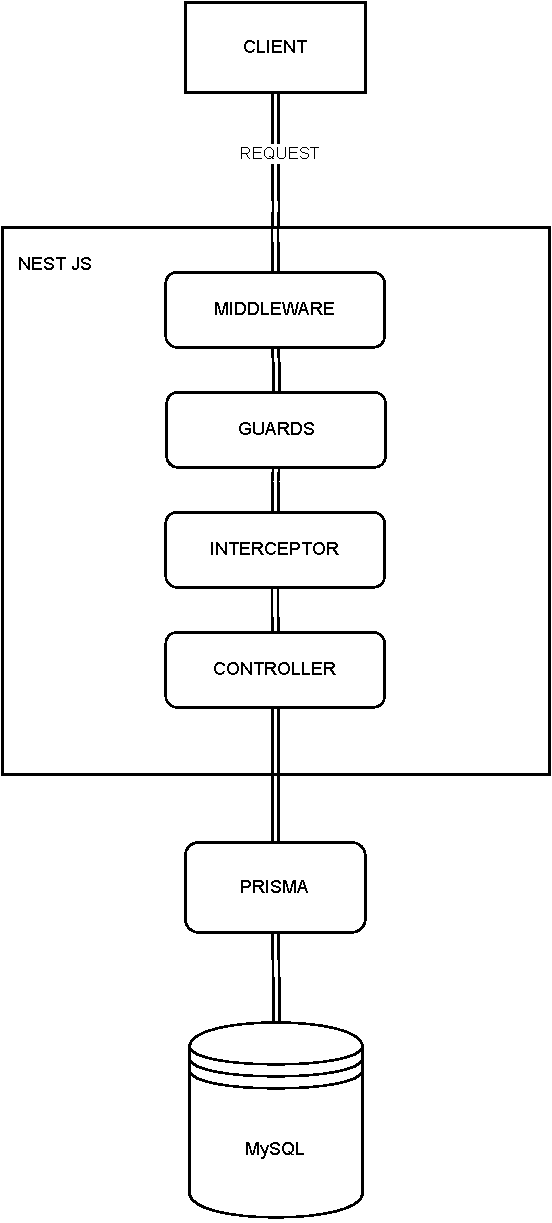
\includegraphics[width=0.35\textwidth]{drawio/sistem-desain.drawio.pdf}
	\caption{Desain Sistem}
	\label{sistem-desain}
\end{figure}
\begin{figure}[h]
	\centering
	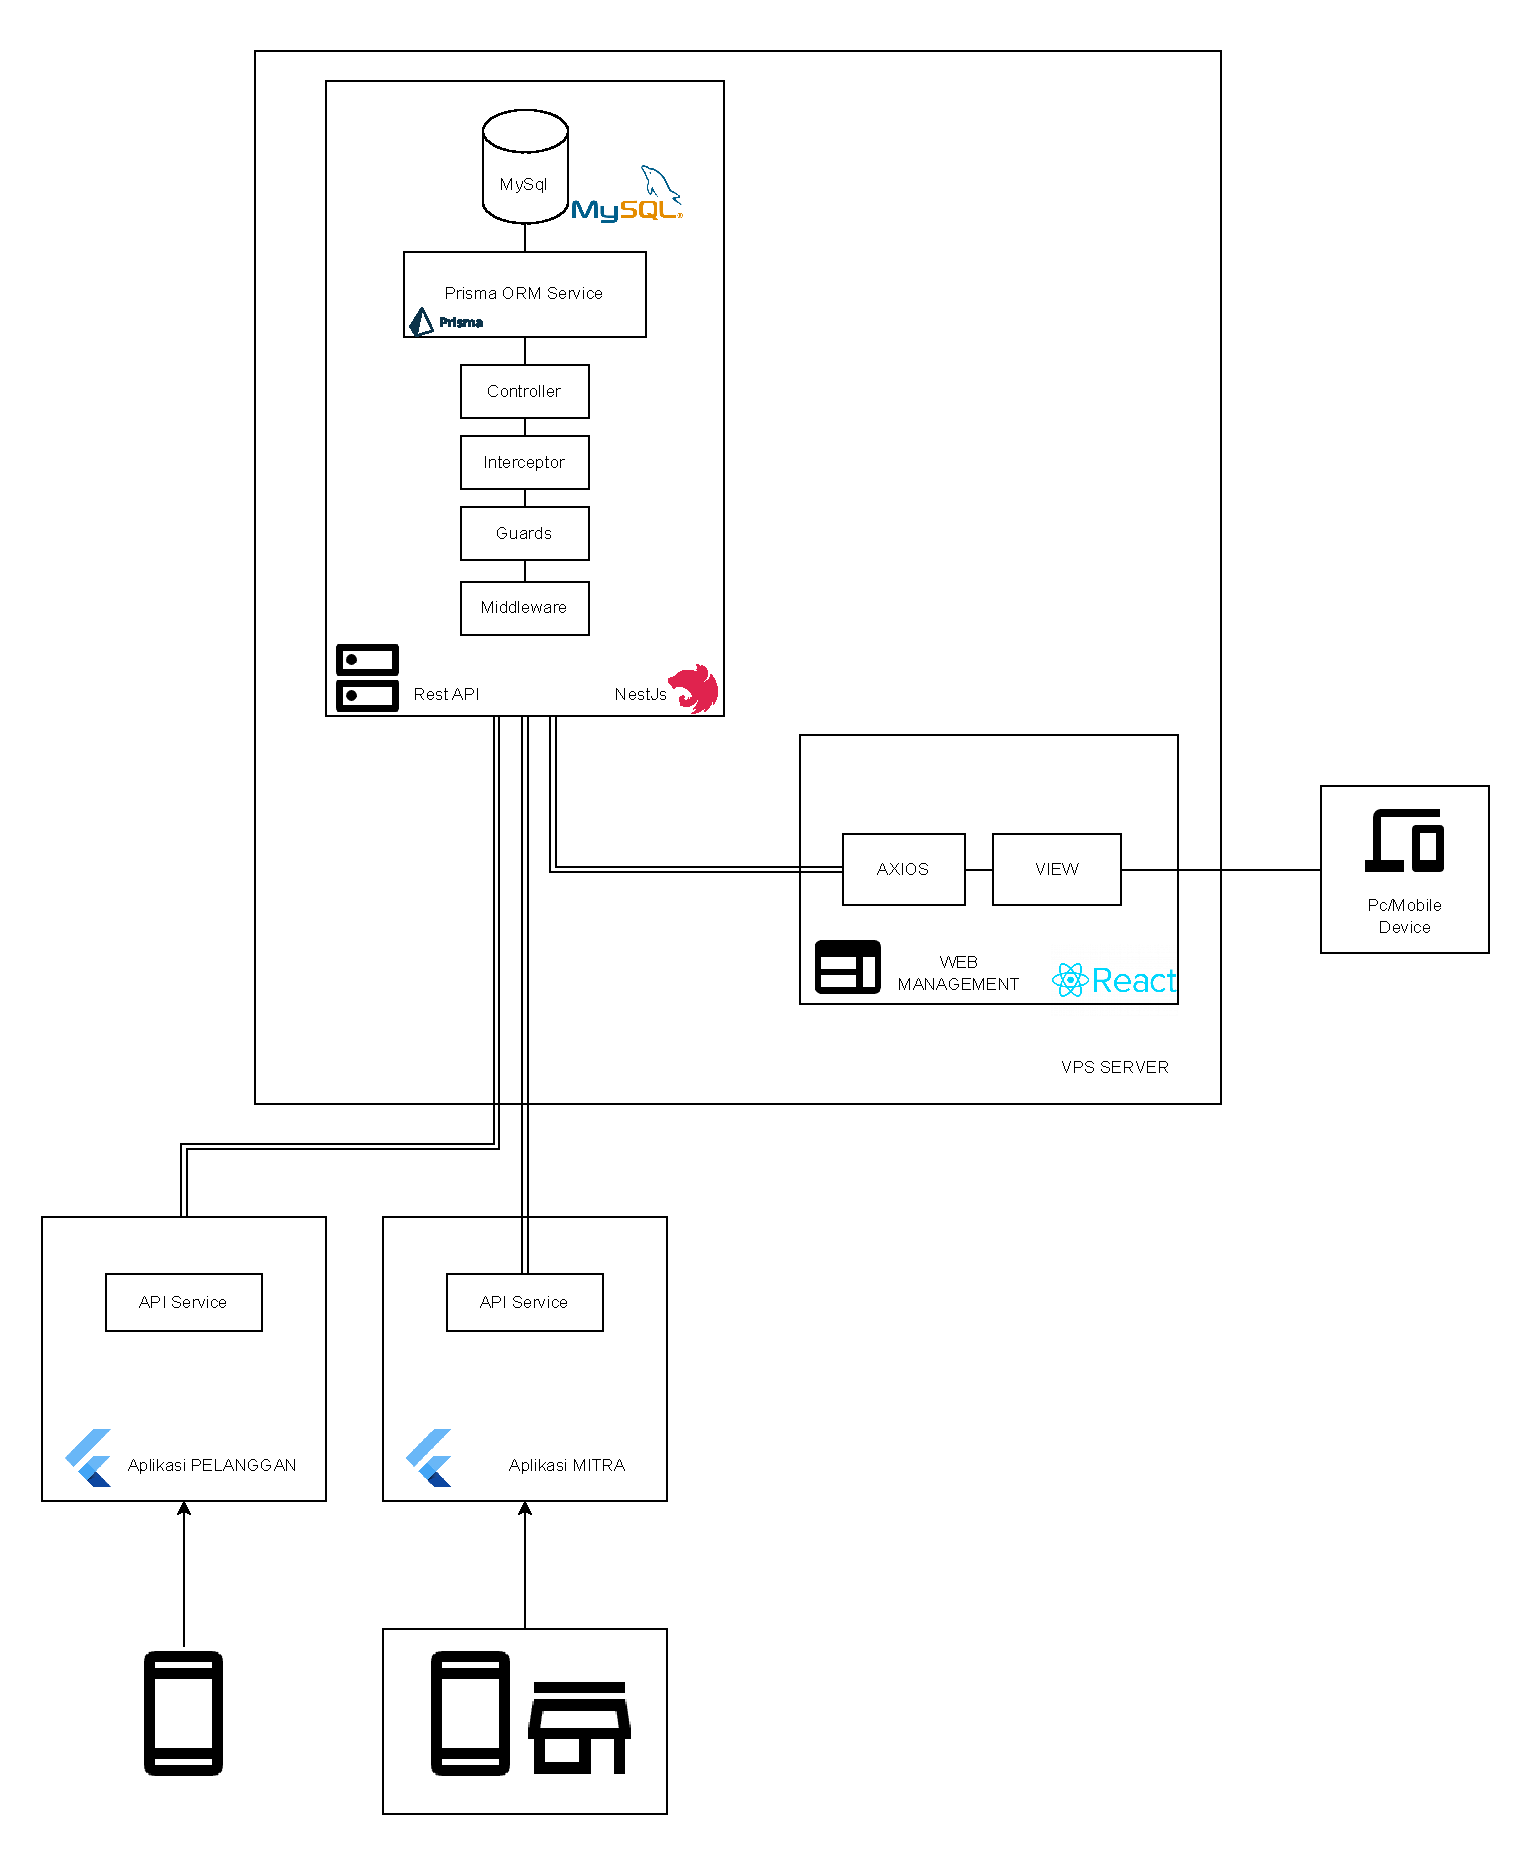
\includegraphics[width=0.73\textwidth]{drawio/System-Design-Architecture.drawio.pdf}
	\caption{Arsitektur Desain Sistem}
	\label{sistem-desain-arsitektur}
\end{figure}

\newpage
\subsection{Middleware}
Pada Middleware, fungsi akan dipanggil sebelum masuk ke routing. fungsi middleware dapat mengakses data \textit{request} dan \textit{response}. beberapa fungsi Middleware seperti \textit{logger}, dan cek notifikasi. Contoh penggunaan nya bisa seperti
\begin{lstlisting}[caption={Middleware},label={lst:middleware}]
  export class LoggerMiddleware implements NestMiddleware {
    use(req: Request, res: Response, next: NextFunction) {
      console.log('Request...');
      next();
    }
  }  
\end{lstlisting}

\subsection{Guard}
Pada Guard, \textit{request} akan dicek \textit{authenticity}, untuk mengetahui validitas dari \textit{request} tersebut. Tahap ini juga akan dicek keamanan session menggunakan JWT dan CSRF. Contoh penggunaan guard seperti
\begin{lstlisting}[caption={Penggunaan Guards pada Controller},label={lst:guard}]
  @UseGuards(AuthGuard)
  @Get('profile')
  getProfile(@Request() req) {
      return req.user;
  }
\end{lstlisting}


\subsection{Interceptor}
Setelah melalui Guard, Request akan masuk ke Interceptor. Dimana jika suatu \textit{request} mempunyai suatu karakteristik yang ditentukan, maka akan menjalankan fungsi tambahan. Interceptor terjadi ketika \textit{request} datang \textit{(pre)}, dan response \textit{(post)}. Contoh implementasi Interceptor
\begin{lstlisting}[caption={Interceptor},label={lst:interceptor}]
  @UseInterceptors(FileInterceptor('profile_picture',fileInterceptor()))
  async update(@Param('id') id: string, @Body() data: Karyawan, @UploadedFile() file: Express.Multer.File): Promise<Karyawan> {}
\end{lstlisting}

\subsection{Controller}
Setelah melewati Interceptor, fungsi di Controller akan dijalankan. Jika pada Controller tersebut perlu data dari database maka akan turun ke service PrismaJs.
\begin{lstlisting}[caption={Controller},label={lst:controller}]
  @Controller('karyawan')
  @Post()
  async create(@Body() data: any): Promise<Karyawan> {
    const hashedPassword = await bcrypt.hash(data.password, 10);
    const karyawanData = { ...data, password: hashedPassword };
    return this.karyawanService.createKaryawan(karyawanData);
  }
\end{lstlisting}

\subsection{Service}
Pada Service, fungsi akan melakukan database call menggunakan ORM ke database MySQL yang akan di kembalikan (return) ker Controller\cite{NestJS}. Contoh implementasi service
\begin{lstlisting}[caption={Service},label={lst:service}]
  async karyawans(params: {
    skip?: number;
    take?: number;
    cursor?: Prisma.KaryawanWhereUniqueInput;
    where?: Prisma.KaryawanWhereInput;
    orderBy?: Prisma.KaryawanOrderByWithRelationInput;
  }): Promise<Karyawan[]> {
    const { skip, take, cursor, where, orderBy } = params;
    return this.prisma.karyawan.findMany({
      skip,take,cursor,where,orderBy,
    });
  }
\end{lstlisting}

\subsection{Deployment}
Ketika backend selesai di develope dan siap dipakai maka akan dilakukan deployment.
Pada diagram \ref{deployment} menjelaskan bagaimana server backend berkomunikasi dengan Aplikasi lain melalui protokol HTTPS. 

\begin{figure}[h]
	{\centering {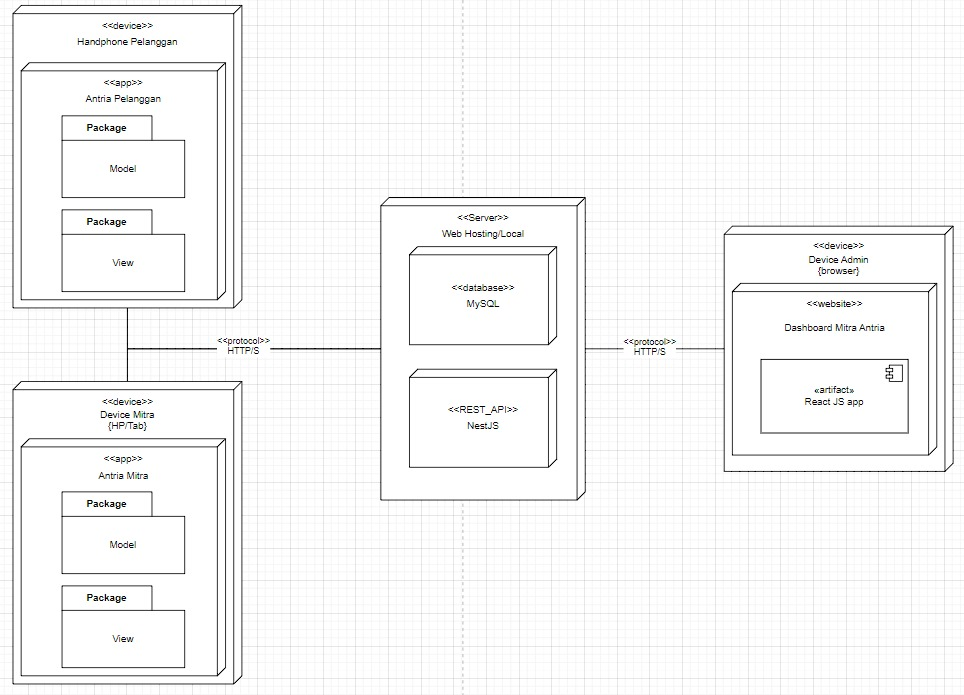
\includegraphics[scale=0.5]{drawio/deployment.jpg}}\par}
	\caption{Deployment Diagram}
	\label{deployment}
\end{figure}


\section{Implementasi dan Evaluasi}

\subsection{Prisma}
Berdasarkan SRS, didapatkan beberapa entity pada database meliputi: Pelanggan, Mitra, Produk, OrderList, Pesanan, Antrian, Karyawan, Review, Chat, dan Analytic.
\begin{lstlisting}[caption={Prisma Scheme},label={lst:scheme}]
model Pelanggan {
  id              Int       @default(autoincrement()) @id
  username        String    @unique
  password        String
  email           String    @unique
  emailVerified   Boolean   @default(false)
  profile_picture String    @default("")
  nama            String
  handphone       String    @default("")
  alamat          String    @default("")
  review          Review[]
  pesanan         Pesanan[]
  chat            Chat[]
  wallet          Int       @default(0)
  created_at      DateTime  @default(now())
  updated_at      DateTime  @updatedAt
}

model Mitra {
  id              Int         @default(autoincrement()) @id
  nama_toko       String      
  deskripsi_toko  String
  alamat          String
  linkGmaps       String      @default("")
  hari_buka       String      
  jam_buka        String
  jam_tutup       String
  gambar_toko     String      @default("")
  subscription    Boolean     @default(false)
  review          Review[]
  produk_layanan  Produk[]
  order           Pesanan[]
  karyawan        Karyawan[]
  chat            Chat[]
  status_toko     StatusToko  @default(OPEN)
  created_at      DateTime    @default(now())
  updated_at      DateTime    @updatedAt
}
model Produk {
  id                Int       @default(autoincrement()) @id
  nama_produk       String
  deskripsi_produk  String 
  harga             Int       
  gambar            String    @default("default.png")
  kuantitas         Int       @default(10)
  mitra             Mitra     @relation(fields: [mitraId], references: [id])
  mitraId           Int
  orderList         OrderList[]
  show_produk       Boolean   @default(true)
  created_at        DateTime  @default(now())
  updated_at        DateTime  @updatedAt
}
model OrderList {
  id        Int       @default(autoincrement()) @id
  quantity  Int       @default(1)
  note      String    @default("")
  pesanan   Pesanan   @relation(fields: [pesananId], references: [invoice])
  produk    Produk    @relation(fields: [produkId], references: [id])
  produkId  Int
  pesananId String
}
model Pesanan {
  invoice     String        @id  
  payment     Payment
  pemesanan   OrderType?    @default(ONLINE)
  takeaway    Boolean       @default(false)
  status      PaymentStatus @default(PENDING)
  oderlist    OrderList[]
  pelanggan   Pelanggan     @relation(fields: [pelangganId], references: [id])
  pelangganId Int
  mitra       Mitra         @relation(fields: [mitraId], references: [id])
  mitraId     Int
  antrian     Antrian?
  antrianId   Int?
  created_at  DateTime      @default(now())
  updated_at  DateTime      @updatedAt
}
model Antrian {
  id          Int         @default(autoincrement()) @id
  estimasi    Int?
  orderstatus OrderStatus @default(WAITING)
  pesanan     Pesanan     @relation(fields: [pesananId], references: [invoice])
  pesananId   String      @unique
  created_at  DateTime    @default(now())
  updated_at  DateTime    @updatedAt
}
model Karyawan {
  id              Int       @default(autoincrement()) @id
  username        String    @unique
  password        String
  email           String    @unique
  profile_picture String    @default("")
  nama            String
  handphone       String    @default("")
  alamat          String    @default("")
  isOwner         Boolean   @default(false)
  mitra           Mitra     @relation(fields: [mitraId], references: [id])
  mitraId         Int
  created_at      DateTime  @default(now())
  updated_at      DateTime  @updatedAt
}
model Review {
  komentar    String
  rating      Int
  mitra       Mitra     @relation(fields: [mitraId], references: [id])
  mitraId     Int
  reviewer    Pelanggan @relation(fields: [pelangganId], references: [id])
  pelangganId Int
  created_at  DateTime  @default(now())
  updated_at  DateTime  @updatedAt  

  @@id([mitraId,pelangganId])
}
model Chat {
  id          Int       @default(autoincrement()) @id
  message     String
  attachment  String?
  pelanggan   Pelanggan @relation(fields: [pelangganId], references: [id])
  pelangganId Int
  mitra       Mitra     @relation(fields: [mitraId], references: [id])
  mitraId     Int
  isRead      Boolean
  created_at  DateTime  @default(now())
  updated_at  DateTime  @updatedAt  
}
model Analytic {
  id    Int     @default(autoincrement()) @id
}
enum Payment {
  EWALLET
  CASH
}
enum OrderStatus {
  ALLDONE
  CONFIRM
  PROCESS
  WAITING
  CANCELED
}
enum PaymentStatus {
  PENDING
  SUCCESS
  FAILED
}
enum OrderType {
  ONLINE
  OFFLINE
}
enum StatusToko {
  OPEN
  CLOSE
  FULL
}
\end{lstlisting}

\subsection{Guards}
implementasi code guards dibuat 2 fungsi, guards untuk pengguna, dan guards untuk mitra.
\begin{lstlisting}[caption={Authentication Guards}, label={lst:authguards}]
  export class AuthGuard implements CanActivate {
    constructor(private jwtService: JwtService) {}
    async canActivate(context: ExecutionContext): Promise<boolean> {
      const request = context.switchToHttp().getRequest();
      const token = this.extractTokenFromHeader(request);
      if (!token) {
        throw new UnauthorizedException();
      }
      try {
        const payload = await this.jwtService.verifyAsync(
          token,
          {
            secret: jwtConstants.secret
          }
        );
        request['user'] = payload;
      } catch {
        throw new UnauthorizedException();
      }
      return true;
    }
  
    private extractTokenFromHeader(request: Request): string | undefined {
      const [type, token] = request.headers.authorization?.split(' ') ?? [];
      return type === 'Bearer' ? token : undefined;
    }
  }
\end{lstlisting}

\subsection{Interceptor}
Interceptor digunakan untuk mengambil file gambar dari request client, lalu disimpan ke dalam file storage server.
\begin{lstlisting}[caption={File Interceptor},label={lst:fileinterceptor}]
  @UseInterceptors(FileInterceptor('profile_picture',{
    storage: diskStorage({
      destination: "./MediaUpload/",
      filename: (req, file, callback) => {
        const uniqueSuffix = uuidv4();
        const fileExtName = path.extname(file.originalname);
        const newFileName = `${uniqueSuffix}${fileExtName}`;
        callback(null, newFileName);
      }
    })
  }))
\end{lstlisting}

\subsection{Controller}
Controller minimal mengikuti banyak entity pada model. masing masing controller memiliki 4 fungsi yang merepresentasikan method http yaitu GET, POST, PUT, DELETE.
\subsubsection{Pelanggan controller}
\subsubsection{Mitra controller}
\subsubsection{Produk controller}
\subsubsection{OrderList controller}
\subsubsection{Pesanan controller}
\subsubsection{Antrian controller}
\subsubsection{Karyawan controller}
\subsubsection{Review controller}
\subsubsection{Chat controller}
\subsubsection{Analytic controller}

\subsection{Service}
Sama seperti controller, banyak service minimal mengikuti banyak entity pada model.
bedanya service berinteraksi langsung dengan ORM Prisma.
\subsubsection{Pelanggan Service}
\subsubsection{Mitra Service}
\subsubsection{Produk Service}
\subsubsection{OrderList Service}
\subsubsection{Pesanan Service}
\subsubsection{Antrian Service}
\subsubsection{Karyawan Service}
\subsubsection{Review Service}
\subsubsection{Chat Service}
\subsubsection{Analytic Service}

\subsection{API Endpoint}
Untuk menghindari Anti Pattern, API endpoint sesuai dengan nama entity pada model.
setiap endpoint entity mendukung 4 method http.
\subsubsection{Auth Endpoint}
Auth merupakan endpoint yang berhubungan dengan autentikasi client.
\begin{longtable}{| p{3.5cm} | p{1.5cm} | p{3cm} | p{3cm} | p{4cm} |}
  \caption{Auth Endpoint Table} \\
  \hline
  \textbf{Path} & \textbf{Method} & \textbf{Description} & \textbf{Parameters} & \textbf{Responses} \\
  \hline
  \endfirsthead
  
  \multicolumn{5}{c}%
  {{\bfseries \tablename\ \thetable{} -- continued from previous page}} \\
  \hline
  \textbf{Path} & \textbf{Method} & \textbf{Description} & \textbf{Parameters} & \textbf{Responses} \\
  \hline
  \endhead
  
  \hline \multicolumn{5}{|r|}{{Continued on next page}} \\ \hline
  \endfoot
  
  \hline
  \endlastfoot
  
  /auth/login/pelanggan & POST &  &  & \\
  \hline
  /auth/login/mitra & POST &  &  & \\
  \hline
  /auth/profile & GET &  &  & \\
  \hline
  
\end{longtable}

\subsubsection{Pelanggan Endpoint}
Endpoint ini berhubungan dengan entity pelanggan pada model prisma.
\begin{longtable}{| p{2.5cm} | p{1.5cm} | p{4cm} | p{3cm} | p{4cm} |}
  \caption{Pelanggan Endpoint Table} \\
  \hline
  \textbf{Path} & \textbf{Method} & \textbf{Description} & \textbf{Parameters} & \textbf{Responses} \\
  \hline
  \endfirsthead
  
  \multicolumn{5}{c}%
  {{\bfseries \tablename\ \thetable{} -- continued from previous page}} \\
  \hline
  \textbf{Path} & \textbf{Method} & \textbf{Description} & \textbf{Parameters} & \textbf{Responses} \\
  \hline
  \endhead
  
  \hline \multicolumn{5}{|r|}{{Continued on next page}} \\ \hline
  \endfoot
  
  \hline
  \endlastfoot
  
  /pelanggan & GET &  &  & \\
  \hline
  /pelanggan & POST &  &  & \\
  \hline
  /pelanggan/\{id\} & GET &  &  & \\
  \hline
  /pelanggan/\{id\} & PUT &  &  & \\
  \hline
  /pelanggan/\{id\} & DELETE &  &  & \\

  \hline
  
\end{longtable}
\subsubsection{Karyawan Endpoint}
Endpoint ini berhubungan dengan entity karyawan pada model prisma.
\begin{longtable}{| p{4.5cm} | p{1.5cm} | p{3cm} | p{3cm} | p{3cm} |}
  \caption{Karyawan Endpoint Table} \\
  \hline
  \textbf{Path} & \textbf{Method} & \textbf{Description} & \textbf{Parameters} & \textbf{Responses} \\
  \hline
  \endfirsthead
  
  \multicolumn{5}{c}%
  {{\bfseries \tablename\ \thetable{} -- continued from previous page}} \\
  \hline
  \textbf{Path} & \textbf{Method} & \textbf{Description} & \textbf{Parameters} & \textbf{Responses} \\
  \hline
  \endhead
  
  \hline \multicolumn{5}{|r|}{{Continued on next page}} \\ \hline
  \endfoot
  
  \hline
  \endlastfoot
  
  /karyawan & GET &  &  & \\
  \hline
  /karyawan & POST &  &  & \\
  \hline
  /karyawan/\{id\} & GET &  &  & \\
  \hline
  /karyawan/\{id\} & PUT &  &  & \\
  \hline
  /karyawan/\{id\} & DELETE &  &  & \\
  \hline
  /karyawan/mitra/\{mitraId\} & GET &  &  & \\
  \hline
  
\end{longtable}

\subsubsection{Mitra Endpoint}
Endpoint mitra
\begin{longtable}{| p{2cm} | p{1.5cm} | p{4.5cm} | p{3cm} | p{4cm} |}
  \caption{Mitra Endpoint Table} \\
  \hline
  \textbf{Path} & \textbf{Method} & \textbf{Description} & \textbf{Parameters} & \textbf{Responses} \\
  \hline
  \endfirsthead
  
  \multicolumn{5}{c}%
  {{\bfseries \tablename\ \thetable{} -- continued from previous page}} \\
  \hline
  \textbf{Path} & \textbf{Method} & \textbf{Description} & \textbf{Parameters} & \textbf{Responses} \\
  \hline
  \endhead
  
  \hline \multicolumn{5}{|r|}{{Continued on next page}} \\ \hline
  \endfoot
  
  \hline
  \endlastfoot
  
  /mitra & GET &  &  & \\
  \hline
  /mitra & POST &  &  & \\
  \hline
  /mitra/\{id\} & GET &  &  & \\
  \hline
  /mitra/\{id\} & PUT &  &  & \\
  \hline
  /mitra/\{id\} & DELETE &  &  & \\
  \hline
  
\end{longtable}

\subsubsection{Produk Endpoint}
Endpoint produk
\begin{longtable}{| p{3.5cm} | p{1.5cm} | p{4cm} | p{3cm} | p{3cm} |}
  \caption{Produk Endpoint Table} \\
  \hline
  \textbf{Path} & \textbf{Method} & \textbf{Description} & \textbf{Parameters} & \textbf{Responses} \\
  \hline
  \endfirsthead
  
  \multicolumn{5}{c}%
  {{\bfseries \tablename\ \thetable{} -- continued from previous page}} \\
  \hline
  \textbf{Path} & \textbf{Method} & \textbf{Description} & \textbf{Parameters} & \textbf{Responses} \\
  \hline
  \endhead
  
  \hline \multicolumn{5}{|r|}{{Continued on next page}} \\ \hline
  \endfoot
  
  \hline
  \endlastfoot
  
  /produk & GET &  &  & \\
  \hline
  /produk & POST &  &  & \\
  \hline
  /produk/\{id\} & GET &  &  & \\
  \hline
  /produk/\{id\} & PUT &  &  & \\
  \hline
  /produk/\{id\} & DELETE &  &  & \\
  \hline
  /produk/mitra/\{mitraId\} & GET &  &  & \\
  \hline
  
\end{longtable}

\subsubsection{Pesanan Endpoint}
pesanan endpoint

\begin{longtable}{| p{4cm} | p{1.5cm} | p{3.5cm} | p{3cm} | p{3cm} |}
  \caption{Pesanan Endpoint Table} \\
  \hline
  \textbf{Path} & \textbf{Method} & \textbf{Description} & \textbf{Parameters} & \textbf{Responses} \\
  \hline
  \endfirsthead
  
  \multicolumn{5}{c}%
  {{\bfseries \tablename\ \thetable{} -- continued from previous page}} \\
  \hline
  \textbf{Path} & \textbf{Method} & \textbf{Description} & \textbf{Parameters} & \textbf{Responses} \\
  \hline
  \endhead
  
  \hline \multicolumn{5}{|r|}{{Continued on next page}} \\ \hline
  \endfoot
  
  \hline
  \endlastfoot
  
  /pesanan & GET &  &  & \\
  \hline
  /pesanan & POST &  &  & \\
  \hline
  /pesanan/\{invoice\} & GET &  &  & \\
  \hline
  /pesanan/\{invoice\} & PUT &  &  & \\
  \hline
  /pesanan/\{invoice\} & DELETE &  &  & \\
  \hline
  /pesanan/mitra/\{mitraId\} & GET &  &  & \\
  \hline
  
\end{longtable}

\subsubsection{OrderList Endpoint}
Orderlist endpoint

\begin{longtable}{| p{4cm} | p{1.5cm} | p{3.5cm} | p{3cm} | p{3cm} |}
  \caption{OrderList Endpoint Table} \\
  \hline
  \textbf{Path} & \textbf{Method} & \textbf{Description} & \textbf{Parameters} & \textbf{Responses} \\
  \hline
  \endfirsthead
  
  \multicolumn{5}{c}%
  {{\bfseries \tablename\ \thetable{} -- continued from previous page}} \\
  \hline
  \textbf{Path} & \textbf{Method} & \textbf{Description} & \textbf{Parameters} & \textbf{Responses} \\
  \hline
  \endhead
  
  \hline \multicolumn{5}{|r|}{{Continued on next page}} \\ \hline
  \endfoot
  
  \hline
  \endlastfoot
  
  /orderlist & POST &  &  & \\
  \hline
  /orderlist/\{id\} & GET &  &  & \\
  \hline
  /orderlist/\{id\} & PUT &  &  & \\
  \hline
  /orderlist/\{id\} & DELETE &  &  & \\
  \hline
  /orderlist/invoice/\{invoice\} & GET &  &  & \\
  \hline
  
\end{longtable}

\subsubsection{Antrian Endpoint}
Antrian endpoint
\begin{longtable}{| p{4cm} | p{1.5cm} | p{3.5cm} | p{3cm} | p{3cm} |}
  \caption{Antrian Endpoint Table} \\
  \hline
  \textbf{Path} & \textbf{Method} & \textbf{Description} & \textbf{Parameters} & \textbf{Responses} \\
  \hline
  \endfirsthead
  
  \multicolumn{5}{c}%
  {{\bfseries \tablename\ \thetable{} -- continued from previous page}} \\
  \hline
  \textbf{Path} & \textbf{Method} & \textbf{Description} & \textbf{Parameters} & \textbf{Responses} \\
  \hline
  \endhead
  
  \hline \multicolumn{5}{|r|}{{Continued on next page}} \\ \hline
  \endfoot
  
  \hline
  \endlastfoot
  
  /antrian & POST &  &  & \\
  \hline
  /antrian/\{id\} & GET &  &  & \\
  \hline
  /antrian/\{id\} & PUT &  &  & \\
  \hline
  /antrian/\{id\} & DELETE &  &  & \\
  \hline
  /antrian/mitra/\{mitraId\} & GET &  &  & \\
  \hline
  
\end{longtable}

\subsubsection{Reviews Endpoint}
Reviews endpoint
\begin{longtable}{| p{5cm} | p{1.5cm} | p{3.5cm} | p{3cm} | p{2cm} |}
  \caption{Reviews Endpoint Table} \\
  \hline
  \textbf{Path} & \textbf{Method} & \textbf{Description} & \textbf{Parameters} & \textbf{Responses} \\
  \hline
  \endfirsthead
  
  \multicolumn{5}{c}%
  {{\bfseries \tablename\ \thetable{} -- continued from previous page}} \\
  \hline
  \textbf{Path} & \textbf{Method} & \textbf{Description} & \textbf{Parameters} & \textbf{Responses} \\
  \hline
  \endhead
  
  \hline \multicolumn{5}{|r|}{{Continued on next page}} \\ \hline
  \endfoot
  
  \hline
  \endlastfoot
  /reviews & GET &  &  & \\
  \hline
  /reviews & POST &  &  & \\
  \hline
  /reviews/mitra/\{mitraId\} & GET &  &  & \\
  \hline
  /reviews/\{mitraId\}/\{pelangganId\} & GET &  &  & \\
  \hline
  /reviews/\{mitraId\}/\{pelangganId\} & PUT &  &  & \\
  \hline
  /reviews/\{mitraId\}/\{pelangganId\} & DELETE &  &  & \\
  \hline
  
\end{longtable}

\subsubsection{Image server endpoint}
endpoint berikut untuk menyajikan gambar ke client
\begin{longtable}{| p{3cm} | p{1.5cm} | p{4.5cm} | p{3cm} | p{3cm} |}
  \caption{Image server Endpoint Table} \\
  \hline
  \textbf{Path} & \textbf{Method} & \textbf{Description} & \textbf{Parameters} & \textbf{Responses} \\
  \hline
  \endfirsthead
  
  \multicolumn{5}{c}%
  {{\bfseries \tablename\ \thetable{} -- continued from previous page}} \\
  \hline
  \textbf{Path} & \textbf{Method} & \textbf{Description} & \textbf{Parameters} & \textbf{Responses} \\
  \hline
  \endhead
  
  \hline \multicolumn{5}{|r|}{{Continued on next page}} \\ \hline
  \endfoot
  
  \hline
  \endlastfoot
  /image/\{fileName\} & GET &  &  & \\
  \hline
  
\end{longtable}

\subsection{Hasil Pengujian}

Pertama, tampilkan hasil pengujian yang paling utama. Kemudian hasil-hasil yang lebih detil ditampilkan setelah hasil yang utama. Mengingat tinggi atau rendah, baik atau jeleknya hasil pengujian bersifat relatif, maka sangat dianjurkan ada pembanding (baseline) yang membandingkan dengan algoritma atau pendekatan yang dipilih untuk TA. Pembanding dijalankan pada lingkungan (termasuk data set) yang sama.

Pilih tabel atau jenis diagram yang sesuai untuk menampilkan hasil pengujian. 


\subsection{Analisis Hasil Pengujian}
 Analisis merupakan salah satu bagian yang penting untuk TA. Pada TA S1 tidak dituntut untuk mendapatkan hasil performasi yang lebih bagus dibandingkan dengan baseline yang populer, yang dituntut adalah membuat analisis yang lengkap. Menganalisis pengaruh kondisi-kondisi yang berbeda (seperti parameter, jenis data, threshold, dan sub-sistem) yang digunakan. 
 
 Cara sitasi adalah sebagai berikut: \citep{van2002fundamentals} untuk buku, \citep{ochoa2003hybrid} untuk \textit{paper}, dan \citep{Budi} untuk website.
   
   
\section{Kesimpulan}
 \noindent Bagian Kesimpulan memuat kesimpulan dan Saran (\textit{Future Work}), bisa dituliskan dalam poin-poin ataupun paragraf-paragraf. Semua poin kesimpulan diambil dari hasil pengujian dan analisis hasil pengujian sehingga tidak ada kesimpulan dari teori ataupun nalar semata. Sebagaimana sudah disebutkan pada bagian sebelumnya, pengujian dan analisis harus sesuai dengan tujuan TA. Jadi kesimpulan-kesimpulan yang dituliskan selaras dengan seluruh tujuan TA. 
 


\bibliographystyle{abbrv}
\bibliography{references}

\section*{Lampiran}

\noindent Lampiran dapat berupa detil data dan contoh lebih lengkapnya, data-data pendukung, detail hasil pengujian, analisis hasil pengujian, detail hasil survey, surat pernyataan dari tempat studi kasus, screenshot tampilan sistem, hasil kuesioner dan lain-lain.